\documentclass[aspectratio=169,12pt]{beamer}
\usepackage[T1]{fontenc}
\usepackage{lmodern,tikz}
\definecolor{Ink}{HTML}{17324D}
\definecolor{Teal}{HTML}{007F7B}
\definecolor{Gray}{HTML}{697887}
\definecolor{Soft}{HTML}{EEF3F6}
\setbeamercolor{normal text}{fg=Ink,bg=white}
\setbeamercolor{frametitle}{fg=Ink}
\setbeamercolor{structure}{fg=Teal}
\setbeamercolor{block title}{fg=white,bg=Teal}
\setbeamercolor{block body}{fg=Ink,bg=Soft}
\setbeamertemplate{navigation symbols}{}
\setbeamersize{text margin left=9mm,text margin right=9mm}
\setbeamerfont{frametitle}{size=\Large,series=\bfseries}
\setbeamertemplate{footline}{\hspace{9mm}\scriptsize Preliminary research | Alex Towell\hfill\insertframenumber/4\hspace{9mm}\vspace{3mm}}
\newcommand{\aside}[1]{\vfill{\footnotesize\color{Gray}#1\par}}
\hypersetup{pdftitle={Learning to choose steps and use tools},pdfauthor={Alex Towell}}
\begin{document}

\begin{frame}[t]
\frametitle{How can a model solve an unfamiliar task?}
We want a language model to discover useful steps, use tools, and check whether the job is finished.
\medskip

\textbf{A simple test: make a pickaxe in a crafting game.}
\begin{center}
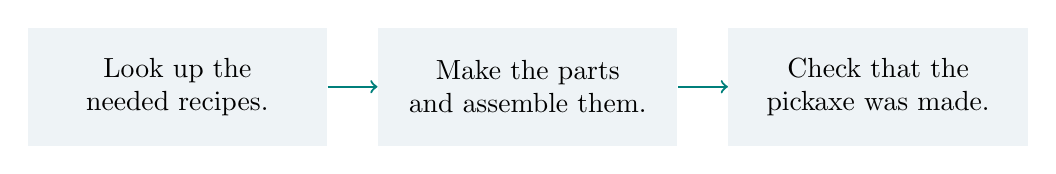
\begin{tikzpicture}[every node/.style={font=\normalsize,align=center},box/.style={fill=Soft,text width=3.45cm,minimum height=1.5cm,inner sep=5pt}]
\node[box] (a) at (0,0) {Look up the\\needed recipes.};
\node[box] (b) at (4.45,0) {Make the parts\\and assemble them.};
\node[box] (c) at (8.9,0) {Check that the\\pickaxe was made.};
\draw[->,thick,Teal] (a)--(b);
\draw[->,thick,Teal] (b)--(c);
\end{tikzpicture}
\end{center}
The game checks actual success, not whether the answer sounds convincing.
\medskip

The larger idea is a \textbf{recursive language model (RLM)}: a model that can use code and ask helper models to solve smaller parts.
\aside{Simplified example. Our recent crafting experiments use one model with tools; they do not yet test recursive helper calls.}
\end{frame}

\begin{frame}[t]
\frametitle{We tried learning from success and failure.}
In \textbf{reinforcement learning (RL)}, the model tries answers or actions, receives a score, and learns from the feedback.
\begin{block}{We saw some gains, but not reliable progress in planning.}
Some models answered or selected information better. The gains often weakened on new examples, or did not clearly beat more learning from worked examples.
\end{block}
\textbf{One possible difficulty:} A model can make wrong parts, recover, and finish the pickaxe. A reward for finishing does not identify which earlier actions helped.
\medskip

\textbf{Open question:} How can we reward useful decisions along the way?
\aside{The pickaxe story illustrates why final success may not identify helpful steps. It is not a proven explanation of all our RL results.}
\end{frame}

\begin{frame}[t]
\frametitle{Two recent findings suggest a useful division of work.}
\begin{block}{Teach the model how to find the steps.}
We trained models to imitate worked examples. Examples from a program that discovered recipes worked better than examples from one that already knew them.
\end{block}
Both programs showed recipe lookups; they differed in how they found the sequence of actions.
\begin{block}{Let code handle exact details.}
The model still chose what to make. When code filled in ingredients from an already-read recipe, more tasks succeeded---without extra model training.
\end{block}
\textbf{Choosing a useful step and executing it correctly are different problems.}
\aside{Preliminary results in one crafting game. The teaching examples differ in several ways, so the reason for their advantage is not yet isolated.}
\end{frame}

\begin{frame}[t]
\frametitle{Can better tools make learning easier?}
Our working idea is to let code handle exact details so that learning can focus on choosing useful steps.
\medskip

\textbf{Next, test the idea on new problems.} Does code help both kinds of trained model? Does the advantage from discovery examples remain?
\medskip

\textbf{Then return to RL.} Does this clearer division of work make it easier to learn from success and failure?
\medskip

\textbf{Longer term:} Learn when to ask a helper and when to break a task into smaller parts again.
\begin{block}{For discussion}
What other multi-step task would make this a useful and convincing result?
\end{block}
\aside{Broader tests are queued; improved RL and learned helper use remain open questions.}
\end{frame}
\end{document}
